\documentclass[../../main.tex]{subfiles}
\begin{document}

\begin{flushright}
\footnotesize\textit{【自動文字起こし・要確認】}
\end{flushright}

{\bf [解]}
\subparagraph{$1^\circ$ $(a,b)=(0,0)$の時}

題意は成立．

\subparagraph{$2^\circ$ $a=0,\ b\ne0$の時}

$a^2x^2+b^2y^2\le1$をみたす$(x,y)$は，$x$：任意，$|y|\le1/|b|$であり，$1\le b$であれば良い．

\subparagraph{$3^\circ$ $a\ne0,\ b=0$}

$2^\circ$と同様に$1\le a$であれば良い．

以下，$ab\ne0$のもとで考える．この時，$xy$平面上で$a^2x^2+b^2y^2\le1$のグラフ上の点が$a(x-1)+b(y-1)\le0$をみたすような$(a,b)$の範囲をもとめれば良い．$(x,y)=\left(\dfrac{r}{a}C,\dfrac{r}{b}S\right)$（$C=\cos\theta,\ S=\sin\theta,\ 0\le\theta<2\pi,\ 0\le r\le1$）とおける．これに代入して
\begin{align}
\begin{split}
rC-a+rS-b&\le0 \\
r\sqrt{2}\sin\left(\theta+\dfrac{\pi}{4}\right)&\le a+b
\end{split}
\end{align}
が任意の$\theta,r$で成立すれば良く，その条件は
\begin{align}
a+b\ge\sqrt{2}
\end{align}
以上まとめて，
\begin{align}
a=b=0 \ \text{or}\ (ab\ne0\wedge a+b\ge\sqrt{2})\ \text{or}\ (a=0\wedge b\ge1)\ \text{or}\ (b=0\wedge a\ge1)
\end{align}
図示して下図斜線部（境界，$\bullet$を含む）．

\begin{figure}[htb]
\begin{center}
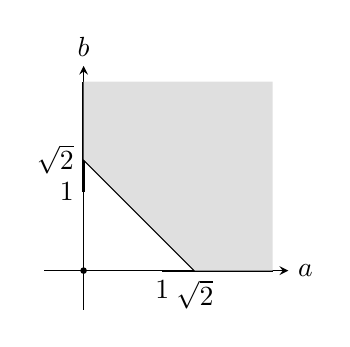
\begin{tikzpicture}[scale=1.0, >=stealth]
  % 座標軸
  \draw[->] (-0.5,0) -- (2.6,0) node[right] {$a$};
  \draw[->] (0,-0.5) -- (0,2.6) node[above] {$b$};
  % 境界: a+b=sqrt2 (ab!=0の場合), a軸上a>=1 (b=0の場合), b軸上b>=1 (a=0の場合)
  \draw[thick] (1.414,0) -- (0,1.414);
  \draw[thick] (1,0) -- (2.4,0);
  \draw[thick] (0,1) -- (0,2.4);
  % 求める領域 a+b>=sqrt2 (a,b>0)
  \fill[gray!25] (1.414,0) -- (0,1.414) -- (0,2.4) -- (2.4,2.4) -- (2.4,0) -- cycle;
  % 原点も条件をみたす
  \fill (0,0) circle (1.2pt);
  \node[below] at (1,0) {$1$};
  \node[below] at (1.414,0) {$\sqrt{2}$};
  \node[left] at (0,1) {$1$};
  \node[left] at (0,1.414) {$\sqrt{2}$};
\end{tikzpicture}
\end{center}
\caption{条件を満たす$(a,b)$の領域（斜線部）}
\end{figure}


\bigskip
\noindent\textbf{[別解]}

{\bf [別解]}
同様に$a\ne0,b\ne0$で考える．$X=ax,\ Y=by$とおく．$x^2+y^2\le1$をみたす全ての$X,Y$が$X+Y\le a+b$をみたせば良く，
\begin{align}
a+b\ge\sqrt{2}
\end{align}
である．


\newpage

\end{document}
